It is of primary interest to apply the \gls{qmla} algorithm to real-life, experimental systems. 
In this chapter we devise an \gls{es} to operate in conjunction with experimental data 
    in order to characterise an electron spin in an \gls{nv} centre in diamond.
In particular, we model, through Hamiltonian terms, interactions between the spin and 
    the spin bath in which it resides,
    so that \gls{qmla} is finding an effective model for the open system dynamics.


\section{\gls{nv}-centres}
\begin{figure}
    \label{fig:nv_centre_energy_levels}
    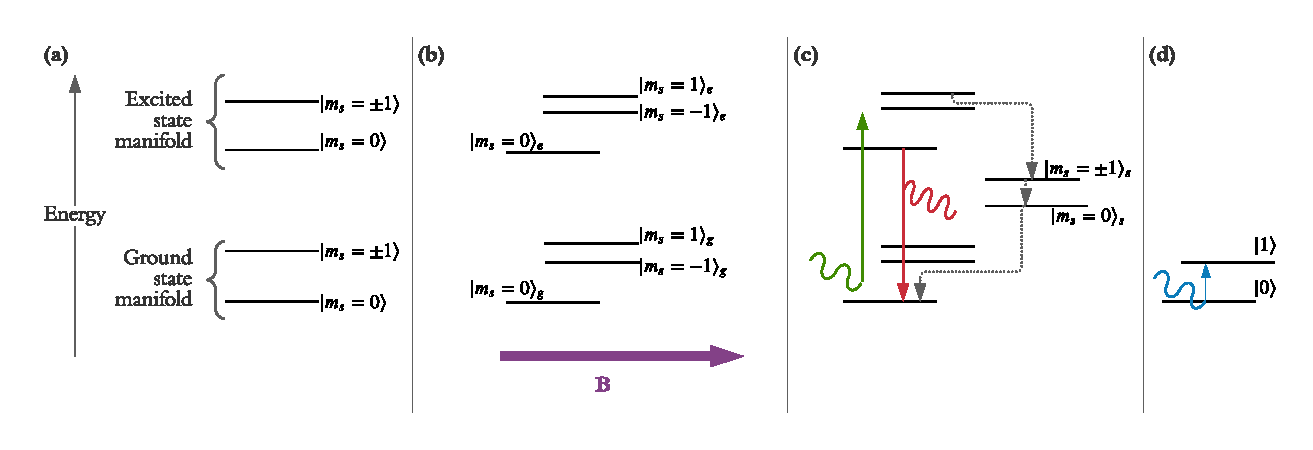
\includegraphics[width=\linewidth]{experimental_study/figures/nv_centre_cartoon.pdf}
    \caption[\glsentrylong{nvc} energy levels.]{
        \glsentrylong{nvc} energy levels. 
        \textbf{a}, With no external field, the system simply has excited and ground-state manifolds, 
        each of which consist of two energy levels depending on the magnetic spin, $m_s$.
        \textbf{b}, In the presence of a magnetic field (purple, $B$), the magnetic spins have distinct energy levels, 
        i.e. hyperfine splitting. States are denoted by their magnetic spin and subscripted by their manifold. 
        \textbf{c},  Application of a green ($637nm$) laser excites the \gls{nvc} from any of the states in the 
        ground state manifold to the excited manifold. 
        The dominant decay mechanism for the excited states are shown: 
            (i) $\ket{m_s=0}_e \rightarrow \ket{m_s=0}_g$ (red line) through the emission of a red photon;
            (ii) $\ket{m_s=\pm 1}_e \rightarrow \ket{m_s=0}_g$ (dotted grey lines) via the shelving manifold which allows for non-spin-preserving transition, 
            and does not emit a photon. 
        \textbf{d}, Computational basis states $\ket{0}$ and $\ket{1}$ are assigned to the two lowest energy states.
            The difference in energy between these states is such that a microwave (MW, blue) photon
            can trigger transition from $\ket{0}$ to $\ket{1}$. 
    }
\end{figure}

\gls{nv} centers are point defects in diamond, 
    occuring naturally or synthetically.
A \gls{nitrogen} isotope is embedded in a lattice of carbon atoms in diamond, 
    specifically such that the \gls{nitrogen} is in a cluster with 
    three \gls{carbon} isotopes as well as a lattice vacancy. 
Of the \gls{nitrogen} atom's five valence electrons, three bond with nearby \glspl{carbon};
    the remaining two unbonded electrons form a \emph{lone pair} in the lattice.
Such systems consisting of two spin-$\frac{1}{2}$ particles have been thoroughly studied\todo{reference}; 
    of particular interest are the resultant triplet states, 
    i.e. the allowed permutations of the two electrons with total quantum spin $S=1$, 
    with magnetic spin multiplicity allowing $m_s = {-1, 0, 1}$, giving rise to distinct energy levels
    for the system. 
In the absence of a magnetic field, the states corresponding to $\ket{m_s=\pm1}$ are degenerate, 
    but in the presence of a magnetic field, $B$, they have distinct energy levels, 
    referred to as hyperfine splitting. 

\par 


A \emph{manifold} is a set of states differing only slightly, 
    for example states near the absolute ground state manifold might differ only in magnetic spin quantum number,
    and can be characterised as the ground state manifold. 
We consider two principle manifolds of the system:
    the ground state and excited manifolds, each consisting of 
    three states, corresponding to the magnetic spin $m_s$. 
For brevity, we denote states with reference to their magnetic spin and manifold, 
    e.g. the state in the ground state manifold with $m_s=0$ is denoted $\ket{m_s=0}_g$. 
\par 

We designate the state $\ket{m_s=0}_g$ as the basis state $\ket{0}=\icol{1 \\ 0}$, 
    and $\ket{m_s=-1}_g$ as $\ket{1}=\icol{0 \\ 1}$, 
    such that we have defined a qubit and computational basis.
By shining a laser of $637$nm (green) on the \gls{nvc}, it is excited to the excited manifold, 
    from which it decays back to the ground state manifold. 
Importantly, the process of this decay can be exploited for the preparation of the \gls{nvc} in 
    the computational basis state $\ket{0}$. 
That is, the dominant decay process from $\ket{m_s=0}_e$ is 
    spin-preserving, so it ends in $\ket{m_s=0}_g$. 
On the other hand, had the \gls{nvc} been in the $\ket{m_s=\pm1}_e$,
    the dominant decay process is through a shelving (singlet) state, 
    and does not preserve spin, such that it also decays to the $\ket{m_s=0}_g$.
Therefore, irrespective of the initial state, 
    by shining the green laser on the \gls{nvc}, 
    it is most likely that it has been prepared in $\ket{m_s=0}_g = \ket{0}$, 
    providing us a starting point from which to perform computation.
\par 

We can further exploit the decay mechanism to compose a readout procedure, 
    to infer the population of $\{\ket{0}, \ket{1}\}$ at a given instant, 
    for example following the application of gates to the system. 
We know that the excitation due to the green laser is spin-preserving, 
    i.e. when the \gls{nvc} is in $\ket{m_s=0}_e$, 
    it had originated in $\ket{m_s=0}_g$.
We also know that the decay $\ket{m_s=0}_e \rightarrow \ket{m_s=0}_g$ is spin preserving, with the emission of 
    a red photon: by simply counting the number of photons emitted, we quantify the population of $\ket{0}$
    at the time of query. 
On the contrary, when the $\ket{m_s=-1}_g$ is excited, spin is also preserved, 
    so it goes to $\ket{m_s=-1}_e$;
    but $\ket{m_s=-1}_e$ decays 
    through the shelving state as outlined earlier, 
    \emph{without} the emission of a photon. 
We can hence infer the population of $\ket{m_s=-1}_g$ at the time of query by the fraction of incidents which don't emit a photon.
\par 

In summary then, by assigning basis states $\ket{0}, \ket{1}$ to energy levels of the ground state manifold, 
    we are able to ensure the preparation of the \gls{nvc} in $\ket{0}$ by first shining a green laser on the \gls{nvc}. 
We can then apply microwave radiation to achieve quantum logical gates on the system, 
    and read out the final state of the system, again by shining a green laser
    and observing the emitted photons (\gls{pl}) and inferring the population level of each basis state. 
We represent these concepts in a simplified format in \cref{fig:nv_centre_energy_levels}. 

\section{Target system}
Assuming the magnetic field aligns with the $z$-axis of the spin, 
    the total interactions the spin is subject to are: 
\begin{easylist}[itemize]
    & ground state energy splitting, $\Delta_{gs}$
    
\end{easylist}
\subsection{Short time dynamics}


\section{\glsentrylong{es}}


\begin{figure}
    \label{fig:exp_qmla_analysis}
    \includegraphics[width=0.95\textwidth]{experimental_study/figures/experimental_qmla_analysis.pdf}
    \caption[\gls{qmla} applied to experimental system.]{
        \textbf{a}, 
        The carbon lattice providing the outer environment for the NV centre, along with the
        time evolution of the electron spin state (represented on a Bloch sphere) during the pulses for the Hahn-echo sequences. The final $\pi/2$ pulse is omitted.  
        \textbf{b}, 
        Simulation of 500 independent \gls{qmla} instances, where $\ho$ is chosen randomly. 
        The win rate is reported against the difference $(N_{p}-N^{\prime}_p)$ between the 
        number of parameters in the \gls{qmla}-selected ($\hp$) and true models, respectively. 
        The \emph{under-parameterised} \emph{ (over-parameterised)} class refers to models with less (more) 
        parameters than $\ho$. 
        \emph{Correct} indicates that exactly $\ho$ was found. 
        The \emph{mis-parameterised} class groups models with the same parametrisation cardinality as $\ho$, but different Hamiltonian terms. 
        \textbf{Inset}, Histogram of occurrences of $R^2$ values for each retrieved $\hp$ 
        against a sampling of datapoints from $\ho$, with median $R^2=0.84$ (red dotted line). 
        \textbf{c}, 
        Win rates of top four models (see main text), for 100 \gls{qmla} instances, 
        against both simulated and experimental data. 
        Simulations use $\ho = \SxyzAz$.
        \textbf{d}, 
        Total volume spanned by the parameters' prior across epochs, for the models in \textbf{c}. 
        Shaded areas indicate $66\%$ credible regions. 
        \textbf{e}, 
        Simulated likelihoods reproduced by the model with the highest win rate ($\hat{S}_{x,y,z}\hat{A}_{z}$, turquoise), compared with corresponding NV-centre system experimental data (red-dots, extracted from the observed \gls{pl} {of the first microseconds in Hahn-echo decay}). 
        Error bars smaller than the dots (see Methods).
        \textbf{f}, 
        A single QMLA instance against experimental data in \textbf{e}, depicted as a \gls{cdag}, see Fig.~\ref{fig:Fig1}c.
        The thin end of each edge points to the favoured model; 
        the colour of the edges maps $\log_{10}\mathcal{B}$ as in the bar legend at the bottom. 
        Layer champions \huc are in light brown, whereas the global champion $\hp$  is in orange.    
    }
\end{figure}